\chapter{Results}
\label{sec:results}
The most interesting questions regarding \emph{HELM} are
\begin{itemize}
	\item How well does \emph{HELM} work compared to the iterative methods?
	\item Is \emph{HELM} able to calculate large scale power nets, for which the iterative methods do not converge?
\end{itemize}
To answer these question I have run several experiments. The ones related to the first question can be found in \secref{comparison_algorithms}. To answer the second question I added in \secref{large_scale_powernets} the results of running \emph{HELM} on the german power net in a certain configuration, for which the iterative algorithms do not converge.

\section{Comparison of the Load-flow Algorithms}
\label{sec:comparison_algorithms}

\begin{table}
	\small
	\begin{tabularx}{\textwidth}{|X|p{1.5cm}|p{1.6cm}|p{1.5cm}|p{1.9cm}|}
		\hline
		method & target precision & maximum iterations & datatype size & maximum coefficients \\ \hline
		Current Iteration & 1e-5 & 100 & & \\ \hline
		Newton-Raphson & 1e-5 & 100 & & \\ \hline
		HELM 64 Bit & 1e-5 & & 64 & 50 \\ \hline
		HELM 200 Bit & 1e-5 & & 200 & 100 \\ \hline
		HELM 64 Bit with Current Iteration & 1e-5 & 100 & 64 & 50 \\ \hline
	\end{tabularx}
	\caption{Algorithm parameter for the comparison}
	\label{tab:comparison_parameter}
\end{table}

\begin{figure}
	\centering
	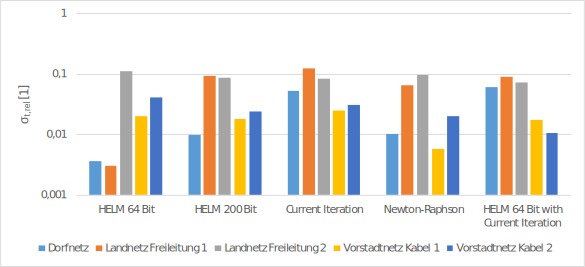
\includegraphics[scale=0.7]{figures/comparison_deviation}
	\caption[Comparison, relative standard deviation of runtime]{Relative standard deviation of the runtime of the algorithms}
	\label{fig:comparison_deviation}
\end{figure}

To compare the different load-flow algorithms I used the sample nets of the Institute and compared the algorithms then regarding their runtime and accuracy. I will not consider the improved convergence behaviour in this section, as I discussed this already in \secref{implementation_helm}. The parameter for the algorithms can be found in \tabref{comparison_parameter}.

To eliminate influences by other processes or the garbage collection on the runtime I ran the calculations five times. The resulting runtimes did not vary much considering the relative standard deviation \figref{comparison_deviation}.

\subsection{Runtime}

\begin{figure}
	\centering
	
\includegraphics[scale=0.7]{figures/comparison_runtime}
	\caption[Comparison, average runtime]{Average runtime of the algorithms for several power nets}
	\label{fig:comparison_runtime}
\end{figure}

One key point is the runtime, and this depends heavily on the implementation of not only the algorithms themselves, but also on the used tools like the library for the sparse linear algebra. Therefore, I am not able to make absolute statements here, especially because I even implemented \emph{HELM} in a different language than the other algorithms. 

The first important message here is only that \emph{HELM} with 64 Bit is considerably fast compared to the \emph{Current Iteration} and \emph{Newton-Raphson}, as it can be seen in \figref{comparison_runtime}. If \emph{Newton-Raphson} runs into convergence problems like in the case of the Vorstadtnetz, \emph{HELM} is even faster than this iterative approach. 

Another conclusion from these tests is that the combination of \emph{HELM} with an iterative method, for instance with the \emph{Current Iteration}, is a very handy approach. In \secref{implementation_helm} I have already shown that this improves the convergence behaviour, but if we also take the runtime into account the combination is not really a drawback. Considering this, I recommend to use always \emph{HELM} with the \emph{Current Iteration} instead of only the later one.

The last important message is the insufficient performance of \emph{HELM} with a datatype bigger than 64 Bit. This setting avoids that floating point operations can be executed within a few clock cycles and therefore deteroiates the performance of the algorithm significantly. Consquently, I recommend to use \emph{HELM} with a bigger datatype only in situations where the calculation with \emph{HELM} with 64 Bit failed.

\subsection{Accuracy}

\begin{figure}
	\centering
	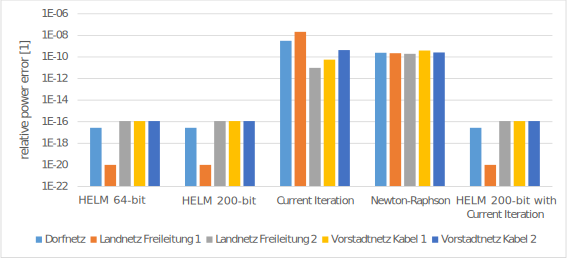
\includegraphics[scale=0.7]{figures/comparison_accuracy}
	\caption[Comparison, accuracy]{Relative power error of the algorithms}
	\label{fig:comparison_accuracy}
\end{figure}

\section{Calculation of Large-Scale Powernets}
\label{sec:large_scale_powernets}

\section{Conclusion}